\documentclass[]{beamer}
%for printing or having a crappy pdf reader backup
%\documentclass[handout]{beamer}
\mode<presentation>
\usetheme{Madrid}


\usecolortheme[RGB={80,0,0}]{structure}
%teal \usecolortheme[RGB={0,128,128}]{structure}
\useoutertheme{miniframes}
\useinnertheme{default}
\usepackage{color}
\definecolor{Maroon}{RGB}{80,0,0}
\definecolor{BurntOrange}{RGB}{204,85,0}
\usepackage{setspace}
\usepackage{amsmath}
\usepackage{amsthm}
\usepackage{amsfonts}
\usepackage{amssymb}
\usepackage{booktabs}
\usepackage{verbatim}
\usepackage{array}
\usepackage{graphicx}
\usepackage{subfigure}
\usepackage{epstopdf}
\usepackage{colortbl}
%\usepackage[retainorgcmds]{IEEEtrantools}
\usepackage{wrapfig}
\usepackage[figurename=,tablename=]{caption}
\usepackage{multirow}
\usepackage[english]{babel}
\usepackage{wasysym}
\usepackage{bigstrut}
\usepackage{textcomp}
%\usepackage{listings}
\usepackage{commath}
\setbeamercolor{normal text}{fg=black}
\setbeamercovered{dynamic}
\beamertemplatetransparentcovereddynamicmedium
%\usepackage{chronology}
\setbeamertemplate{caption}[numbered]

% some simplifying commands
\newcommand{\eg}{{\it e.g.}}
\newcommand{\ie}{{\it i.e.}}
\newcommand{\etal}{{\it et al.}}
\newcommand{\om}{\boldsymbol{\Omega}}

\newlength \figwidth
\setlength \figwidth {0.5\textwidth}
%\setlength{\leftmargin}{-2cm}
%\setlength{\rightmargin}{-2cm}

\begin{document}

\title[Polytope DGFEM Transport]{Higher-Order DGFEM Transport Calculations on Polytope Meshes for Massively-Parallel Architectures}
\author[Hackemack]{{\Large Michael W. Hackemack} \vspace{0.35cm} \\ Chair: {\small Jean C. Ragusa} \\ Committee Members: {\small Marvin L. Adams, Jim E. Morel, Nancy M. Amato } \\ External Advisor: {\small Troy Becker}}
\institute[TAMU]{Department of Nuclear Engineering \\ Texas A\&M University \\ College Station, TX, 77843, USA \\ {\scriptsize mike\_hack@tamu.edu}}
\date[November 24, 2015]

{
\setbeamertemplate{headline}[default] 
\begin{frame}[t]
\vspace{-1.5cm}
	\begin{figure}[t]
		\centering
			\includegraphics[width=.15\textwidth]{images/seal.png}
	\end{figure}
\vspace{-0.55cm}
\titlepage
\end{frame}

}
\begin{frame}
\tableofcontents
\end{frame}

%%%%%%%%%%%%%%%%%%%%%%%%%%%%%%%%%%%%%%%%%%%%%%%%%%%%%%%%%%%%%
%%%%%%%%%%%%%%%%%%%%%%%%%%%%%%%%%%%%%%%%%%%%%%%%%%%%%%%%%%%%%
\section{Overview}
\subsection{}
%---------------------------
\begin{frame}[t]\frametitle{The Continuous-Energy Transport Equation}
\begin{block}{}{\footnotesize
\begin{equation*}
\left[ { \bf \Omega} \cdot {\bf \nabla}  + \sigma_t ({\bf r}, E) \right] \psi ({\bf r}, E, {\bf \Omega}) = \int_{4 \pi} \int_{0}^{\infty}  \, \sigma_s ({\bf r}, E' , E, {\bf \Omega}' , {\bf \Omega}) \psi ({\bf r}, E', {\bf \Omega}') d E'  d \Omega'+ Q ({\bf r}, E, {\bf \Omega})
\end{equation*}
}\end{block}
\begin{block}{} {\footnotesize
${\bf r}$ -  neutron position (cm)\\
$E$ -  neutron energy (eV)\\
${\bf \Omega}$ - neutron solid angle (steradians)\\
$\psi  ({\bf r}, E, {\bf \Omega})$ - angular flux  \\
$Q  ({\bf r}, E, {\bf \Omega})$ - distributed neutron source \\
$\sigma_t ({\bf r}, E)$ - total macroscopic cross section (1/cm)\\
$\sigma_s ({\bf r}, E' , E, {\bf \Omega}' , {\bf \Omega})$ - total 
}\end{block}
\end{frame}
%---------------------------

%---------------------------
\begin{frame}[t]\frametitle{Polytope Grid Motivation}
         \begin{block}{}{\footnotesize
			\begin{itemize}
				\item <1-> Other physics communities are now employing polytope grids due to decreased cell/face counts (CFD in particular)
				\item <2-> They allow for transition elements between different domain regions
				\item <3-> Hanging nodes from non-conforming meshes are not necessary
				\item <4-> Independently-generated simplicial grids ({\em i.e.} created in parallel) can be stitched together with polytopes without communicating the whole mesh across processors
			\end{itemize}}
         \end{block}
	\begin{columns}
	\end{columns}
\end{frame}
%---------------------------
%%%%%%%%%%%%%%%%%%%%%%%%%%%%%%%%%%%%%%%%%%%%%%%%%%%%%%%%%%%%%
%%%%%%%%%%%%%%%%%%%%%%%%%%%%%%%%%%%%%%%%%%%%%%%%%%%%%%%%%%%%%
\section[POLYFEM]{Polytope Finite Element Basis Functions}
\subsection{Linear Basis Functions on 2D Polygons}
%---------------------------
\begin{frame}[t]\frametitle{}
\begin{figure}[t]
\centering
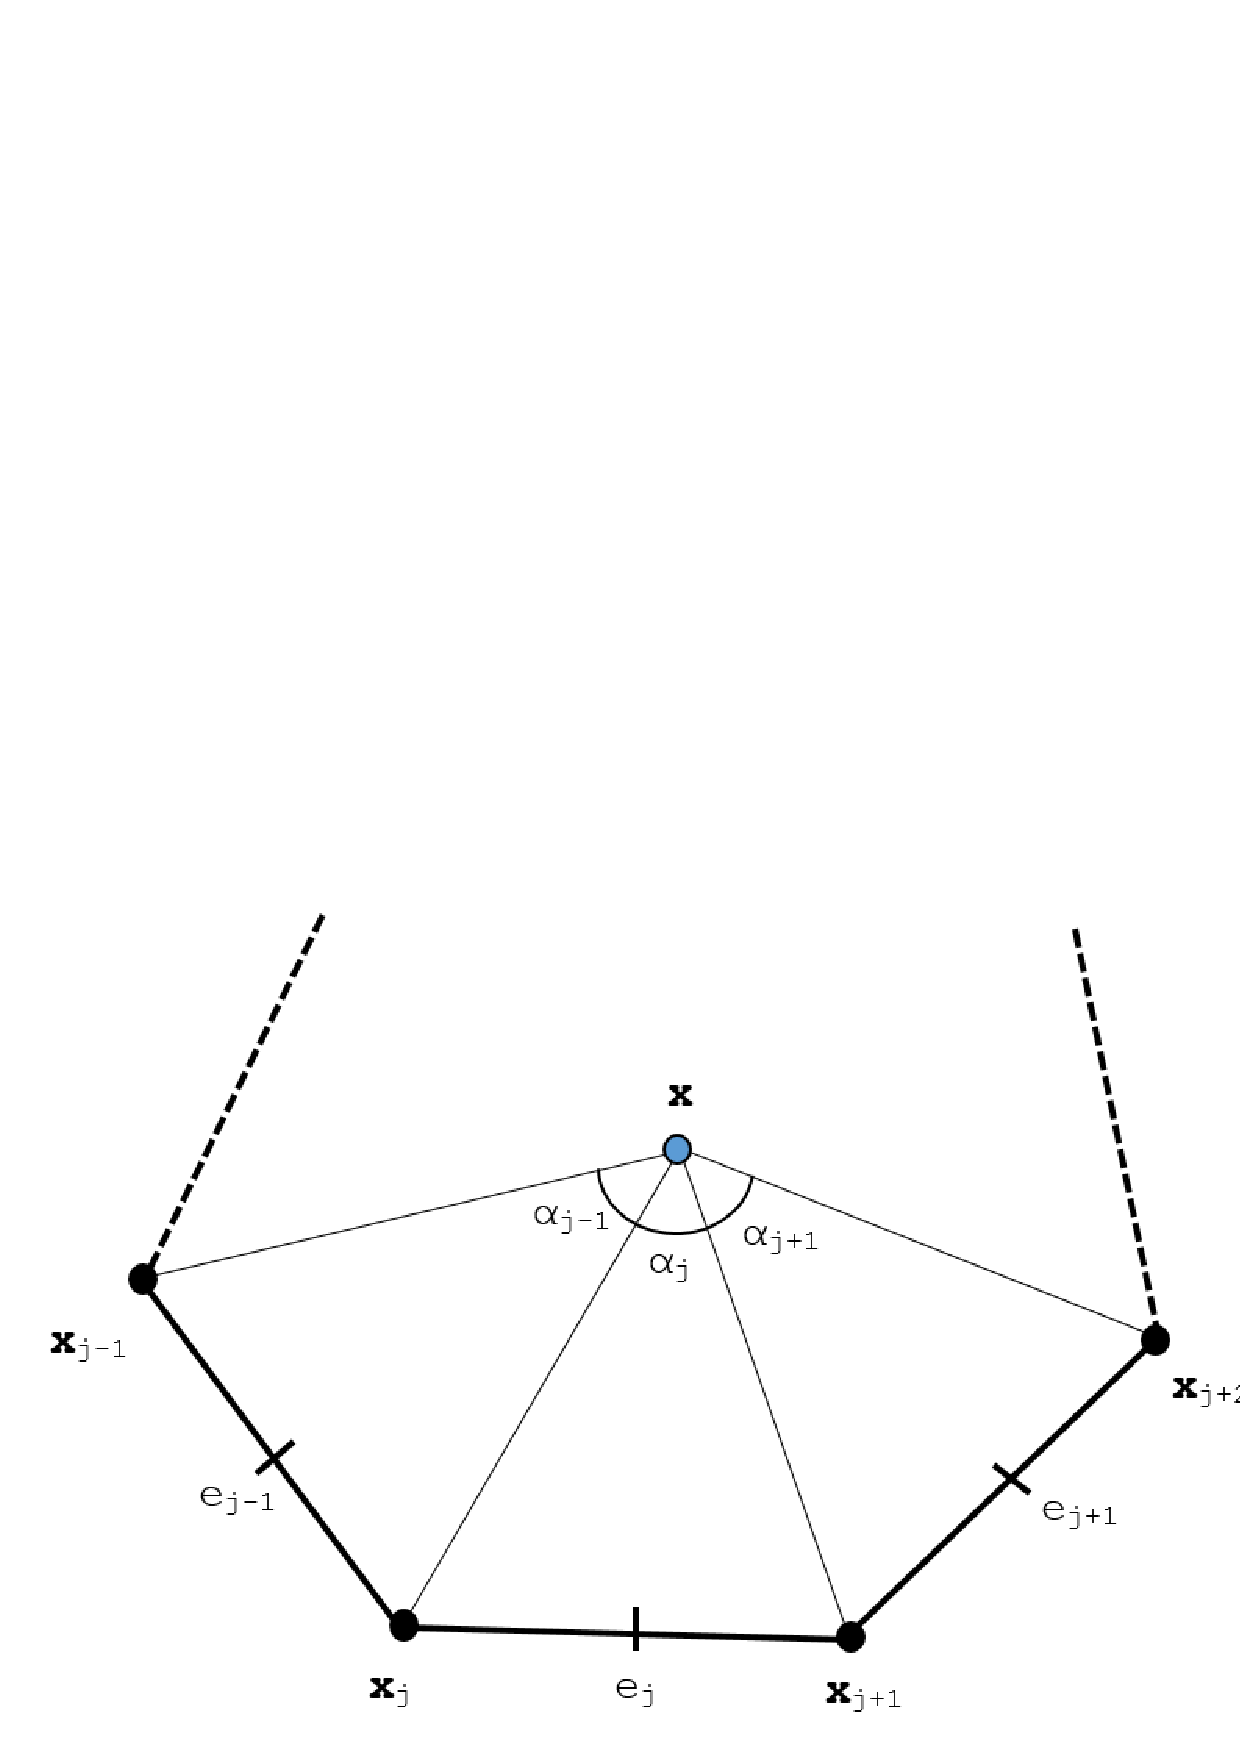
\includegraphics[width=0.45\textwidth]{images/ref_polygon.png}
\end{figure}
\end{frame}
%---------------------------
\begin{frame}[t]\frametitle{Wachspress Rational Functions}

\end{frame}
%---------------------------
\begin{frame}[t]\frametitle{Piecewise Linear Functions}

\end{frame}
%---------------------------
\begin{frame}[t]\frametitle{Mean Value Coordinates}

\end{frame}
%---------------------------
\begin{frame}[t]\frametitle{Maximum Entropy Coordinates}

\end{frame}
%---------------------------
\subsection{Quadratic Serendipity Basis Functions on 2D Polygons}
%---------------------------
\begin{frame}[t]\frametitle{}

\end{frame}
%---------------------------
\subsection{Linear Basis Functions on 3D Polyhedra}
%---------------------------
\begin{frame}[t]\frametitle{}

\end{frame}
%---------------------------
%%%%%%%%%%%%%%%%%%%%%%%%%%%%%%%%%%%%%%%%%%%%%%%%%%%%%%%%%%%%%
%%%%%%%%%%%%%%%%%%%%%%%%%%%%%%%%%%%%%%%%%%%%%%%%%%%%%%%%%%%%%
\section[DSA on Polytopes]{Diffusion Synthetic Acceleration on Polytopes}
\subsection{Theory}
%---------------------------
\begin{frame}[t]\frametitle{}

\end{frame}
%---------------------------
\begin{frame}[t]\frametitle{}

\end{frame}
%---------------------------
\subsection{MIP Diffusion Form}
%---------------------------
\begin{frame}[t]\frametitle{The Diffusion Equation and Boundary Conditions}
	\begin{block}{The Diffusion Equation} {\small 
     		\begin{align*}
 	 		{ \small -{\bf \nabla} \cdot D {\bf \nabla} \Phi ({\bf r}) + \sigma \Phi ({\bf r}) = q ({\bf r}), \qquad  {\bf r} \in \mathcal{D} }
        	\end{align*} }
        	\end{block}
        	\begin{block}{Boundary Conditions} {\small 
		\begin{align*}
 	 		{ \small \Phi ({\bf r})  = \Phi_0 ({\bf r}) , \qquad {\bf r} \in \partial \mathcal{D}^d } \\
 	 		{ \small -D \partial_n \Phi ({\bf r})  = J_0 ({\bf r}) , \qquad {\bf r} \in \partial \mathcal{D}^n } \\
 	 		{ \small \frac{1}{4} \Phi ({\bf r})  + \frac{1}{2}D \partial_n \Phi ({\bf r})  = J^{inc} ({\bf r}) ,  \qquad {\bf r} \in \partial \mathcal{D}^r}
        		\end{align*} }
    \end{block}
\end{frame}
%---------------------------
\begin{frame}[t]\frametitle{Symmetric Interior Penalty (SIP) Form}
	\begin{block}{Bilinear Form}{\small
		\begin{gather*}
			 a( \Phi, b)  = \Big<  D \vec{\nabla}  \Phi , \vec{\nabla} b  \Big>_{\mathcal{D}} + \Big<  \sigma   \Phi ,  b  \Big>_{\mathcal{D}}    \\
			+  \Big\{ \kappa_e^{SIP} [\![   \Phi ]\!] , [\![  b ]\!]\Big\}_{E_h^i} - \Big\{  [\![   \Phi ]\!] , \{\!\{  D \partial_n b \}\!\}\Big\}_{E_h^i} -\Big\{ \{\!\{  D \partial_n  \Phi \}\!\} , [\![ b ]\!]\Big\}_{E_h^i} \\
			+ \Big\{ \kappa_e^{SIP}   \Phi ,   b \Big\}_{\partial \mathcal{D}^d} - \Big\{   \Phi  ,  D \partial_n b \Big\}_{\partial \mathcal{D}^d} - \Big\{   D 				\partial_n  \Phi ,   b \Big\}_{\partial \mathcal{D}^d}  +  \frac{1}{2} \Big\{    \Phi ,   b \Big\}_{\partial \mathcal{D}^r}
        	\end{gather*} }
\end{block}
\begin{block}{Linear Form}{\small
		\begin{align*}
			\ell (b) = \Big<  q, b  \Big>_{\mathcal{D}}  - \Big\{   J_{0}, b  \Big\}_{\partial \mathcal{D}^n} +  2 \Big\{   J_{inc}, b  \Big\}_{\partial 				\mathcal{D}^r} \\ + \Big\{ \kappa_e^{SIP}   \Phi_0 ,   b \Big\}_{\partial \mathcal{D}^d} - \Big\{   \Phi_0  ,  D \partial_n b \Big\}_{\partial 					\mathcal{D}^d} 
        	\end{align*} }
    \end{block}
\end{frame}
%---------------------------
%%%%%%%%%%%%%%%%%%%%%%%%%%%%%%%%%%%%%%%%%%%%%%%%%%%%%%%%%%%%%
%%%%%%%%%%%%%%%%%%%%%%%%%%%%%%%%%%%%%%%%%%%%%%%%%%%%%%%%%%%%%
\section{Proposed Work and Current Status}
\subsection{}
%---------------------------
\begin{frame}[t]\frametitle{}
% ---> linear transport solutions
\end{frame}
%---------------------------
\begin{frame}[t]\frametitle{}
% ---> MMS transport
\end{frame}
%---------------------------
\begin{frame}[t]\frametitle{}
% --->Searchlight problem introduction
\end{frame}
%---------------------------
\begin{frame}[t]\frametitle{}
% --->SL relative outlet error plots
\end{frame}
%---------------------------
\begin{frame}[t]\frametitle{}
% --->SL outgoing flux
\end{frame}
%---------------------------
\begin{frame}[t]\frametitle{}
% --->SL AMR plots with solutions
\end{frame}
%---------------------------
\subsection{}
%---------------------------
\begin{frame}[t]\frametitle{}
% ---> SIP linear solutions on polytopes
\end{frame}
%---------------------------
\begin{frame}[t]\frametitle{}
% ---> SIP MMS results
\end{frame}
%---------------------------
\begin{frame}[t]\frametitle{}
% ---> 2D square fourier analysis
\end{frame}
%---------------------------
\begin{frame}[t]\frametitle{}
% ---> 2D aspect ratio fourier analysis
\end{frame}
%---------------------------
\begin{frame}[t]\frametitle{}
\begin{figure}[t]
\centering
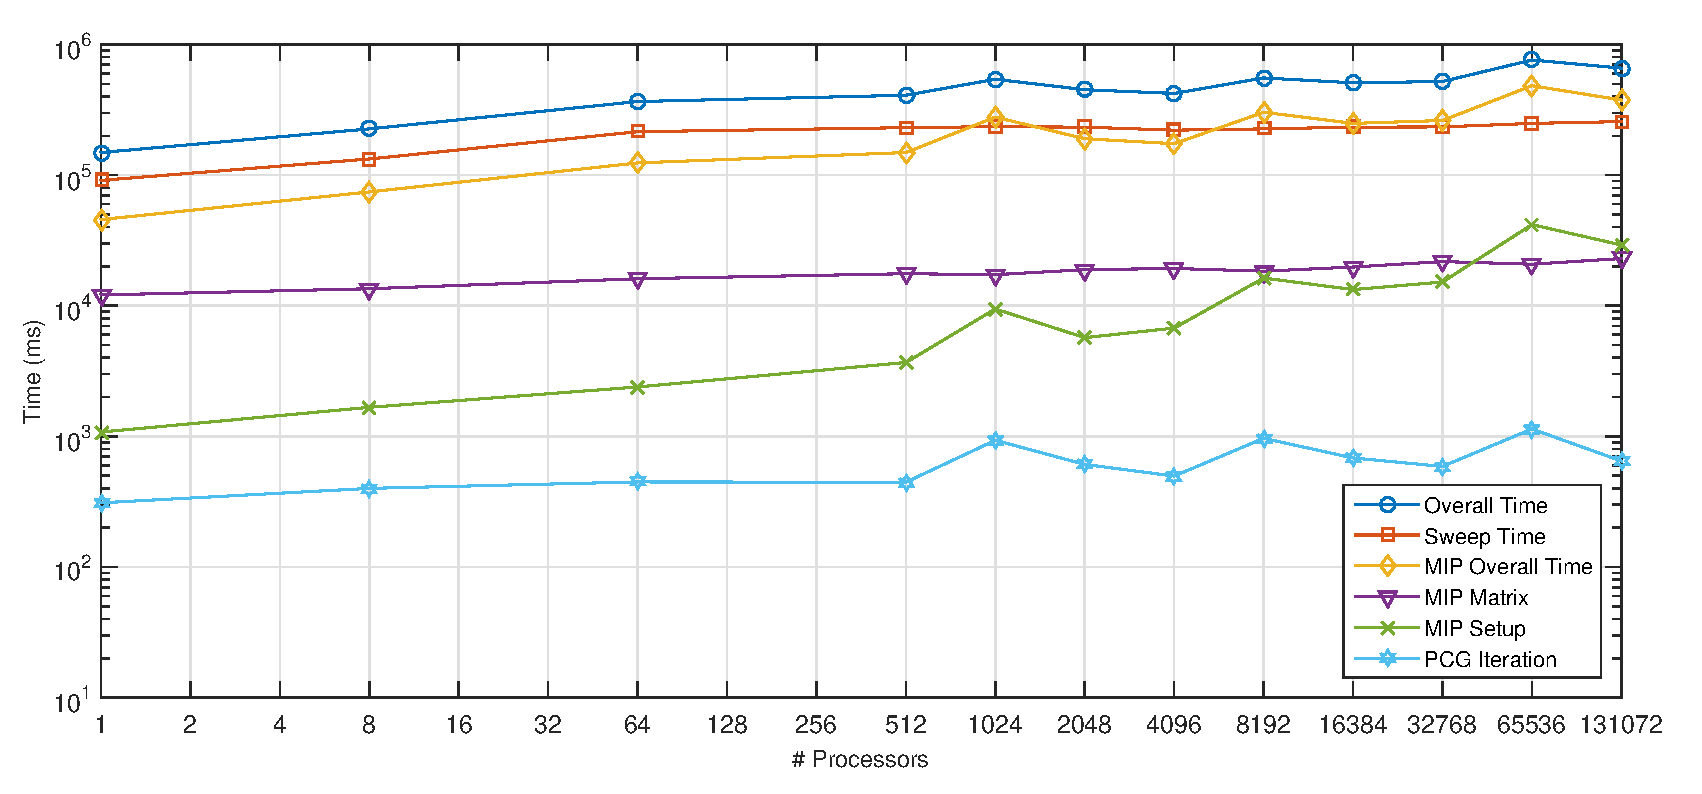
\includegraphics[width=0.95\textwidth]{images/Vulcan_DSA_Timing.eps}
\end{figure}
\end{frame}
%---------------------------
\begin{frame}[t]\frametitle{}
% ---> Vulcan HYPRE parametric study results
\end{frame}
%---------------------------
%%%%%%%%%%%%%%%%%%%%%%%%%%%%%%%%%%%%%%%%%%%%%%%%%%%%%%%%%%%%%
%%%%%%%%%%%%%%%%%%%%%%%%%%%%%%%%%%%%%%%%%%%%%%%%%%%%%%%%%%%%%
\section{Ongoing Work}
\subsection{}
%---------------------------
\begin{frame}[t]\frametitle{}

\end{frame}
%---------------------------
\begin{frame}[t]\frametitle{}

\end{frame}
%---------------------------
\begin{frame}[t]\frametitle{}

\end{frame}
%---------------------------

%%%%%%%%%%%%%%%%%%%%%%%%%%%%%%%%%%%%%%%%%%%%%%%%%%%%%%%%%%%%%
%%%%%%%%%%%%%%%%%%%%%%%%%%%%%%%%%%%%%%%%%%%%%%%%%%%%%%%%%%%%%
\appendix
\section{Additional Material}
\subsection{}
%---------------------------
\begin{frame}[t]\frametitle{}

\end{frame}
%---------------------------
\begin{frame}[t]\frametitle{}

\end{frame}
%---------------------------
\begin{frame}[t]\frametitle{}

\end{frame}
%---------------------------

\end{document}



